% !TEX program = xelatex
\documentclass{article}

% Used packages
\usepackage{geometry}
\usepackage{fancyhdr}
\usepackage{lastpage}
\usepackage[scaled]{helvet}
\usepackage[T1]{fontenc}
\usepackage{hyperref}
\usepackage{indentfirst}
\usepackage{graphicx}
\usepackage{subcaption}

% Document info
\newcommand{\doctitle}{Convolutional Neural Network for Dog Breed Classification}
\newcommand{\docsubtitle}{Udacity Machine Learning Engineer Nanodegree Capstone Project}
\newcommand{\docauthor}{Alex Augusto Costa Machado}
\newcommand{\docdate}{December 10\textsuperscript{th} 2021}

% Page and margin setup
\geometry{
    a4paper,
    left=2cm,
    right=2cm,
    top=2cm,
    bottom=2cm,
    headsep=3mm,
    headheight=1.15cm
    }

% Paragraph setup
\setlength{\parindent}{2.5em}
\renewcommand{\baselinestretch}{1.25}

% Hyperlink setup
\hypersetup{
    colorlinks=true,     
    urlcolor=blue,
    }
    
% Font setup
\renewcommand\familydefault{\sfdefault} 

% Header and footer setup
\pagestyle{fancy}
\fancyhf{}
\rhead{{\doctitle}}
\rfoot{\thepage\ / \pageref*{LastPage}}
\renewcommand{\footrulewidth}{0.4pt}

% First page setup
\newcommand{\docinfo}{
    \thispagestyle{empty}

    \begin{center}

        \Huge\textbf{\doctitle}
        \vspace{2mm}

        \LARGE\textbf{\docsubtitle}
        
        \vspace{3mm}
        \large
        Written by \textbf{\docauthor} on \textbf{\docdate}

    \end{center}
}

% Document
\begin{document}
    \docinfo

    \section{Definition}
    \subsection{Project Overview}

    For computer vision tasks, such as a dog breed classification, an algorithm mostly used is a Convolutional Neural Network, or CNN for short, which is a model that extracts features, like texture and edges, from spatial data.

    The history behind this algorithm started during the 1950s, but it is around the year 2012 that CNNs saw a huge surge in popularity after a CNN called AlexNet achieved state-of-the-art performance labeling pictures in the \href{https://image-net.org/}{ImageNet} challenge. Alex Krizhevsky et al. published the paper "ImageNet Classification with Deep Convolutional Neural Networks" describing the winning AlexNet model.

    \subsection{Problem Statement}

    The purpose of this project is to use a Convolutional Neural Network to classify dog breeds using images as input. For images that contain a human instead of a dog, the algorithm should display which dog breed resembles the human in the picture.

    \subsection{Metrics}

    The metric to evaluate the quality of the classifier is the accuracy of the dog breed predictions. The accuracy can be used in this case because the training data is not imbalanced. The definition of prediction accuracy is as follows:

    \[Accuracy = \frac{TP + TN}{TP +  TN + FP + FN} \]

    Where TP = True Positives, TN = True Negatives, FP = False Positives, and FN = False Negatives.

    \section{Analysis}

    \subsection{Data Exploration}

    There are two datasets for this project: one is a dog dataset containing 8351 images of 133 different dog breeds, and the other is a human dataset consisting of 13233 photos of 5749 different people. The dog dataset is divided in train, validation, and test datasets.

    A sample of the dog dataset is presented in the Figure \ref*{fig:dog_sample}.

    \begin{figure}[htbp]
        \centering
        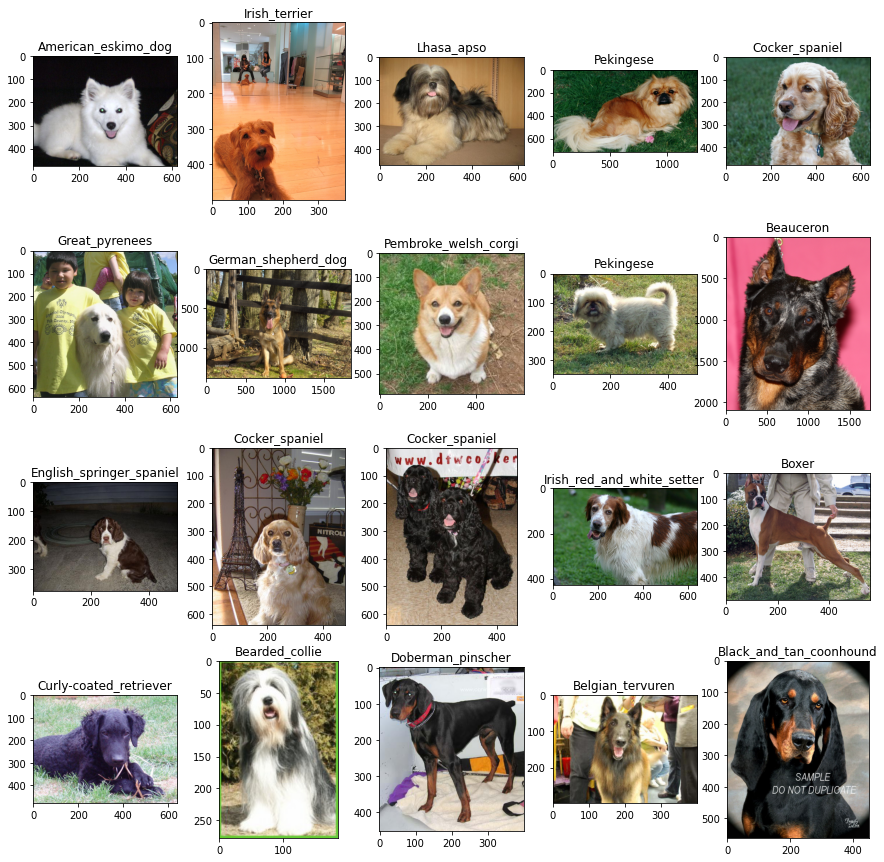
\includegraphics[width=\linewidth]{img/sample.png}
        \caption{Dog dataset sample.}
        \label{fig:dog_sample}
    \end{figure}

    \subsection{Exploratory Visualization}

    A way to explore this image dataset is to verify how many images there are for each of the dog breeds. The Figure \ref*{fig:image_count} presents a graph of image count for each dog breed.

    \begin{figure}[htbp]
        \centering
        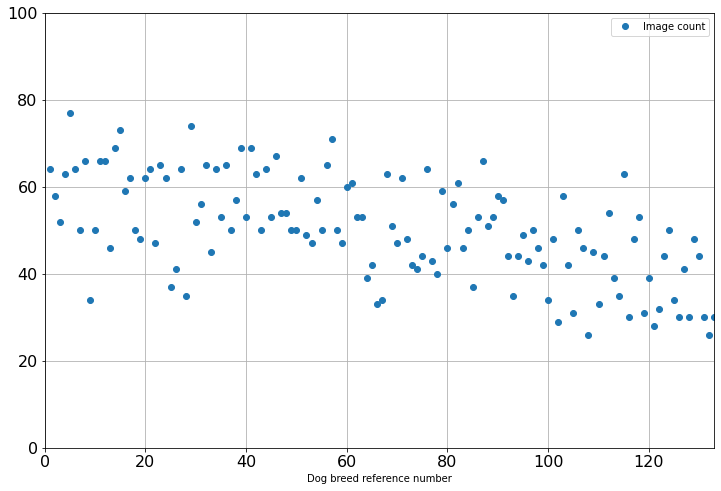
\includegraphics[width=\linewidth]{img/image_count.png}
        \caption{Number of images for each dog breed.}
        \label{fig:image_count}
    \end{figure}
    
    \subsection{Algorithms and Techniques}
    
    Three main algorithms will be used for this project: a human face detector, a dog detector, and a dog breed classifier. More about each of these algorithms is described below.
    
    \begin{itemize}
        \item Human Face Detector: an OpenCV's implementation of Haar feature-based cascade classifier to detect human faces in images. The pre-trained face detector is stored as XML file on \href{https://github.com/opencv/opencv/tree/master/data/haarcascades}{GitHub}.
        
        \item Dog Detector: a pre-trained VGG-16 model with weights that have been trained on \href{https://image-net.org/}{ImageNet}, a very popular dataset used for image classification and other vision tasks.
        
        \item Dog Breed Classifier: a pre-trained VGG-11 model on which the last layer is altered to output 133 classes and trained further using the dog dataset mentioned earlier.
    \end{itemize}
    
    \subsection{Benchmark}
    
    The benchmark for the dog breed classifier will be a simple CNN model designed from scratch that will be compared to the final CNN obtained from transfer learning using a pre-trained VGG-11 model.
    
    The baseline model contains three convolutional blocks, each presenting a convolutional layer, a batch normalization layer and a pooling layer. After these blocks, there is a dropout layer and a fully connected linear layer. A summary of the model is presented on Figure \ref*{fig:model_summary}.
    
    \begin{figure}[htbp]
        \centering
        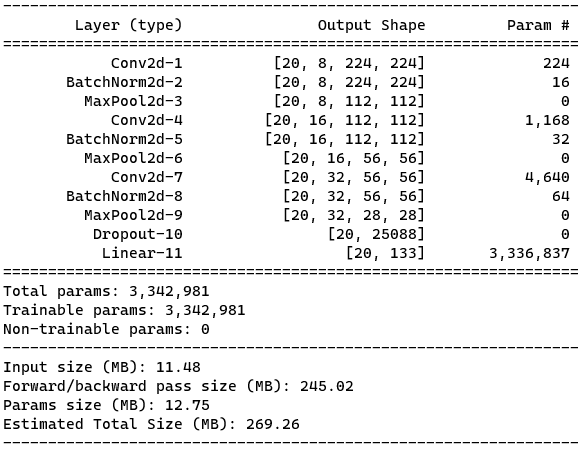
\includegraphics{img/model_summary.png}
        \caption{Summary of the benchmark model.}
        \label{fig:model_summary}
    \end{figure}
    
    \section{Methodology}

    \subsection{Data Preprocessing}

    Since the images have all different sizes, it was necessary to resize them. The images on the validation and testing datasets were resized to 256 pixels and cropped to square shapes of 224x224 pixels about the center and transformed into tensors, then the resulting tensors were normalized. A code snippet is presented on Figure \ref*{fig:transform_train_test}.

    \begin{figure}[htbp]
        \centering
        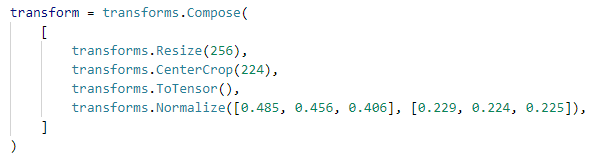
\includegraphics{img/transform_valid_test.png}
        \caption{Code for validation and testing transform.}
        \label{fig:transform_train_test}
    \end{figure}
    
    For the training data, in addition the resizing, cropping and normalization, data augmentation was applied, so the images were also randomly rotated and horizontally flipped. The Figure \ref*{fig:transform_train} presents the code used for this transformation.
    
    \begin{figure}[htbp]
        \centering
        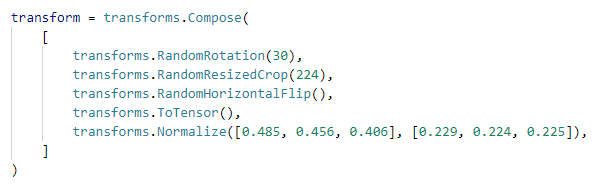
\includegraphics{img/transform_train.png}
        \caption{Code for training transform.}
        \label{fig:transform_train}
    \end{figure}

    \subsection{Implementation}

    The steps required for this implementation are as follow:

    \begin{itemize}
        \item Exploration of both the dog and human datasets in order to verify the quality of the data and if any cleaning was necessary.
        \item Making all the images the same size and normalizing of images.
        \item Apply data augmentation on training dataset such as random horizontal flip and random rotation.
        \item Configuration of pretrained human face detector using a pretrained OpenCV algorithm.
        \item Configuration of pretrained dog detector using a VGG-16 model.
        \item Design of a Convolutional Neural Network to utilize as benchmark model.
        \item Training, validating and testing benchmark model.
        \item Change a pretrained VGG-11 model to output 133 classes, which is the number of dog breeds on the training dataset.
        \item Train this model using the dog dataset to improve its accuracy.
        \item Test the new model and verify final accuracy.
        \item Write an algorithm that receives an image and, using the models described above, verify if it is that of a dog or a human.
        \item Predict which dog breed is in the image or with which dog breed the human in the picture looks like.
    \end{itemize}

    \subsection{Refinement}

    When using transfer learning with the VGG-11 pretrained model, at first it only reached 46\% of accuracy. Even trying to change the hyperparameters and batch size would make no difference on the final accuracy. What really made it reach 86\% was shuffling the training data before feeding it to the model.

    \section{Results}

    \subsection{Model Evaluation and Validation}

    The model achieved a prediction accuracy of 86\% when exposed to the test dataset. Using images of dogs chosen randomly on the Internet, I obtained the results presented on Table \ref*{tab:target_pred}. Only two cases did not obtain the expected result (pictures 5 and 6), but the predicted dog breed is very similar to the target breed.
    
    On Figure \ref*{fig:comparison_wrong} we can see the images for both cases. A Shih tzu (Figure \ref*{fig:shih_tzu}) was provided as input, but a Lhasa apso (Figure \ref*{fig:lhasa}) was predicted. The same happened for the Staffordshire bull terrier (Figure \ref*{fig:staffy}) used as input and the American staffordshire terrier (Figure \ref*{fig:american_staffy}) received as prediction.
    
    \begin{table}[htbp]
        \centering
        \begin{tabular}{c|c|c}
             & \textbf{Target} & \textbf{Prediction} \\
            \hline
            \textbf{Picture 1} & Alaskan malamute & Alaskan malamute \\
            \textbf{Picture 2} & French bulldog & French bulldog \\
            \textbf{Picture 3} & Afghan hound & Afghan hound \\
            \textbf{Picture 4} & Boxer & Boxer \\
            \textbf{Picture 5} & Shih tzu & Lhasa apso \\
            \textbf{Picture 6} & Staffordshire bull terrier & American staffordshire terrier \\
        \end{tabular}
        \caption{Comparison between target values and prediction results.}
        \label{tab:target_pred}
    \end{table}

    \begin{figure}[htbp]
        \centering
        \begin{subfigure}{.35\textwidth}
            \centering
            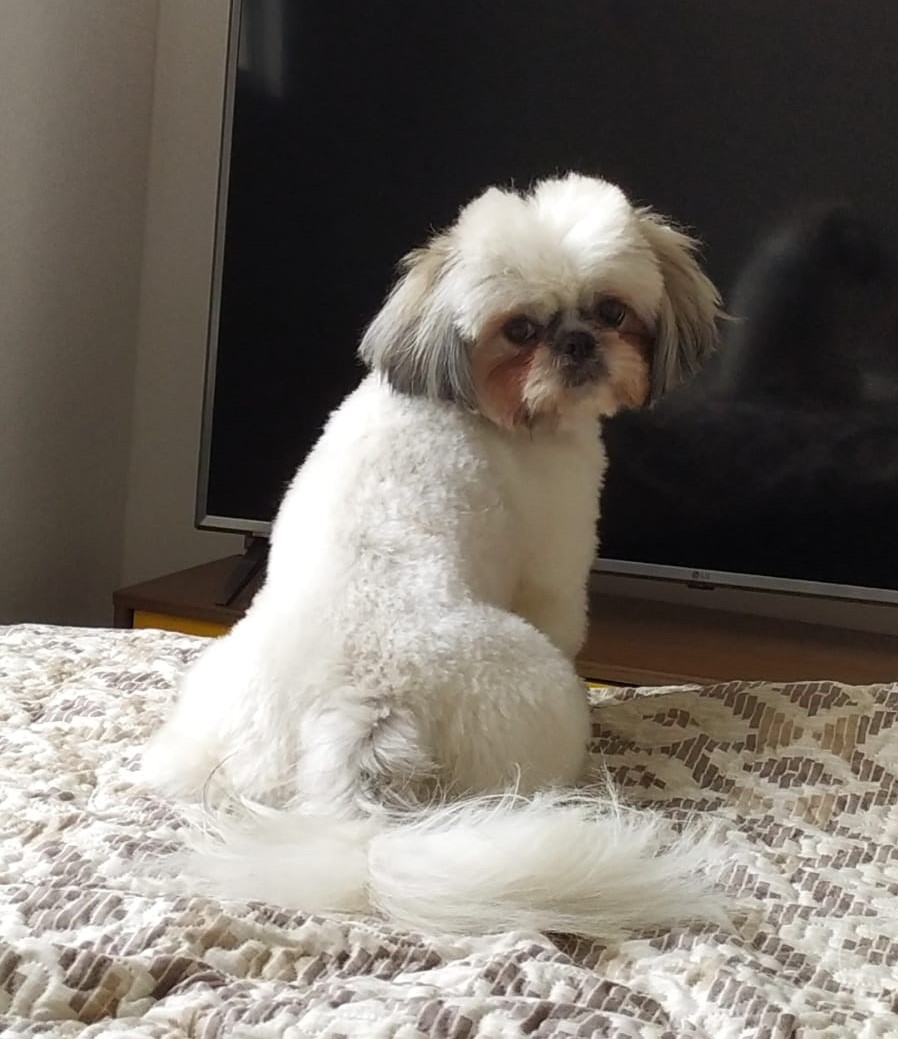
\includegraphics[width=\linewidth]{img/dog_shihtzu.jpeg}
            \caption{Target: Shih tzu}
            \label{fig:shih_tzu}
        \end{subfigure}%
        \hspace{0.1\textwidth}
        \begin{subfigure}{.45\textwidth}
            \centering
            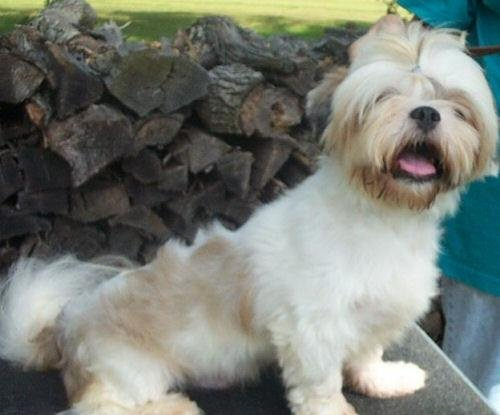
\includegraphics[width=\linewidth]{img/Lhasa_apso_06652.jpg}
            \caption{Prediction: Lhasa apso}
            \label{fig:lhasa}
        \end{subfigure}
        \begin{subfigure}{.35\textwidth}
            \centering
            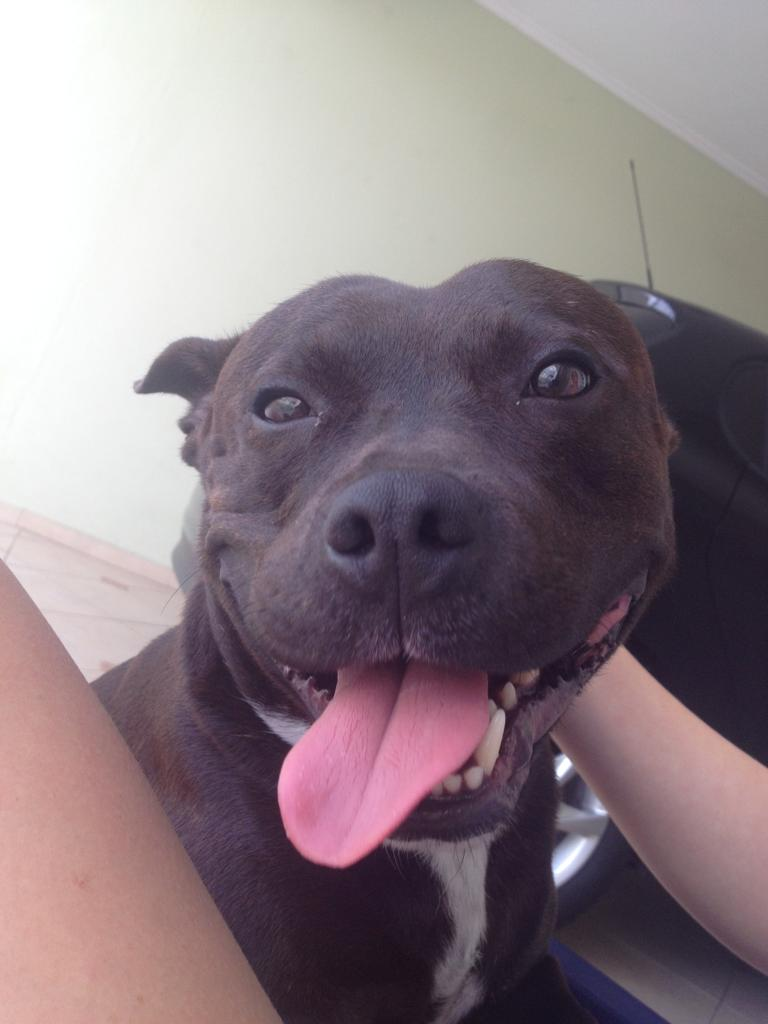
\includegraphics[width=\linewidth]{img/dog_staffordshire_bull_terrier.jpeg}
            \caption{Target: Staffordshire bull terrier}
            \label{fig:staffy}
        \end{subfigure}%
        \hspace{0.1\textwidth}
        \begin{subfigure}{.45\textwidth}
            \centering
            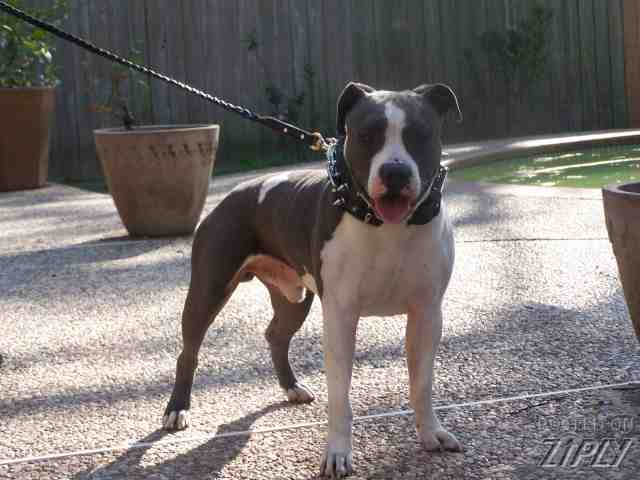
\includegraphics[width=\linewidth]{img/American_staffordshire_terrier_00548.jpg}
            \caption{Prediction: American staffordshire terrier}
            \label{fig:american_staffy}
        \end{subfigure}
        \caption{Comparison for wrongly classified dog breeds.}
        \label{fig:comparison_wrong}
    \end{figure}

    \subsection{Justification}

    The Table \ref*{tab:results_comparison} presents a comparison between the results obtained for the proposed model and the benchmark model.

    \begin{table}[htbp]
        \centering
        \begin{tabular}{c|c|c}
             & \textbf{Benchmark model} & \textbf{Proposed model} \\
            \hline
            \textbf{Epochs} & 80 & 20 \\
            \textbf{Training loss} & 3.437396 & 0.830221 \\
            \textbf{Validation loss} & 3.561250 & 0.534802 \\
            \textbf{Test accuracy} & 20\% & 86\% \\
        \end{tabular}
        \caption{Comparison between benchmark and proposed models.}
        \label{tab:results_comparison}
    \end{table}

    It is possible to see that the proposed model performs a lot better than the benchmark model. As we used transfer learning, the model only required 20 epochs to reach an accuracy of 86\%, which is a satisfactory result.

    \section{Conclusion}

    \subsection{Reflection}

    This project was very important for me to understand the different steps of creating a machine learning model. From data exploration, to preprocessing, training, and testing, all the steps were included in this project.

    The most difficulty I had was making the configuration of the Convolutional Neural Network for the Python program to run correctly without any exceptions being raised.

    \subsection{Improvement}

    Some possible points of improvement are:

    \begin{itemize}
        \item Add functionality to detect dog mutts;
        \item Improve human face detection, as there were human faces detected on some dog images;
        \item Change the algorithm to try and reach over 90\% accuracy.
    \end{itemize}

\end{document}